% =================================================================
% 現代的な日本語レポート・論文用テンプレート（メモ・リファレンス付き）
% =================================================================
% 【注意】コンパイルして日本語が出力されない場合、お使いのエディタの
% 「File/settings/compiler」のCompilerが「LaTeX」になっているか確認してください。

\documentclass{jlreq} % 現代的な日本語標準クラス
\usepackage[dvipdfmx]{graphicx} % 画像サイズ用
\usepackage[top=20truemm, bottom=20truemm, left=15truemm, right=15truemm]{geometry}
\usepackage{float} % 画像配置H用
\usepackage{amsmath} % 計算式記述用(\text や \begin{equation} など)
\usepackage{amssymb}% 数学記号の拡張(\mathbb や \leqslant など)
\usepackage{amsfonts} % 数学フォントの追加(\mathfrak など)
\usepackage{xurl}% referenceどの文字でも自動改行許可

\title{タイトル}
\author{著者名}
\date{\today}

\begin{document}
\maketitle

\begin{abstract}
ここに概要を書きます．
\end{abstract}

\section{はじめに}
文章を書く．先行研究\cite{boominathan2020phlatcam}をここに引用します．

\section{数式例}
行中数式 $E=mc^2$ と別立て式:
$$
\nabla \cdot \mathbf{E} = \frac{\rho}{\varepsilon_0}
$$

\section{図の挿入}
\begin{figure}[H]
  \centering
  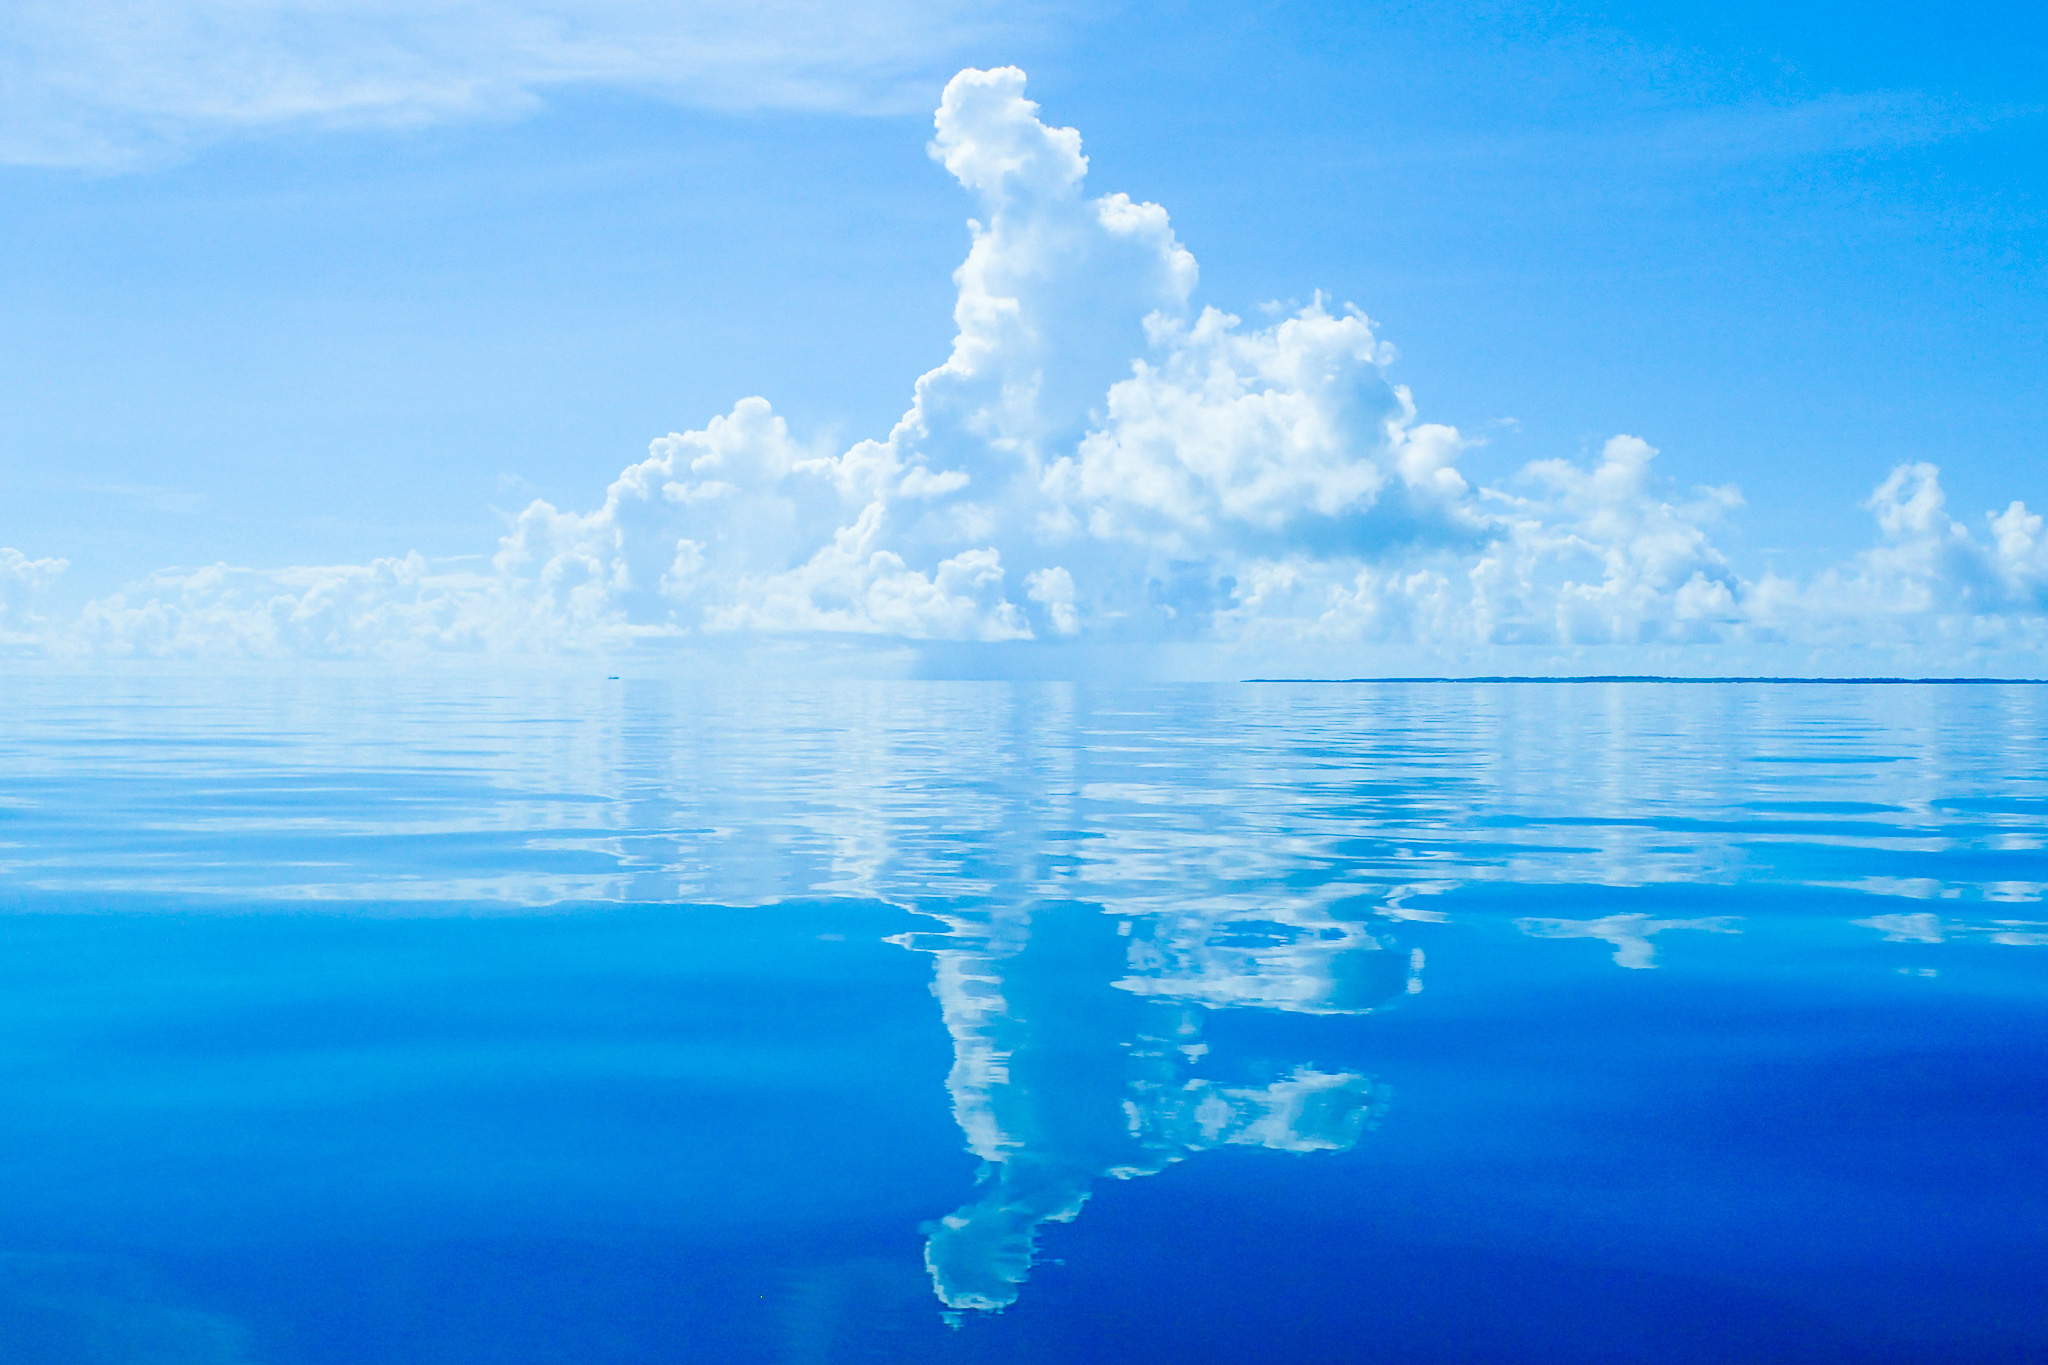
\includegraphics[width=0.6\textwidth]{example.jpg}
  \caption{例の画像}
  \label{fig:example}
\end{figure}

\subsection{図の挿入（続き）}
\begin{figure}[H]
    \centering
    \begin{minipage}[b]{0.32\linewidth}
        \centering
        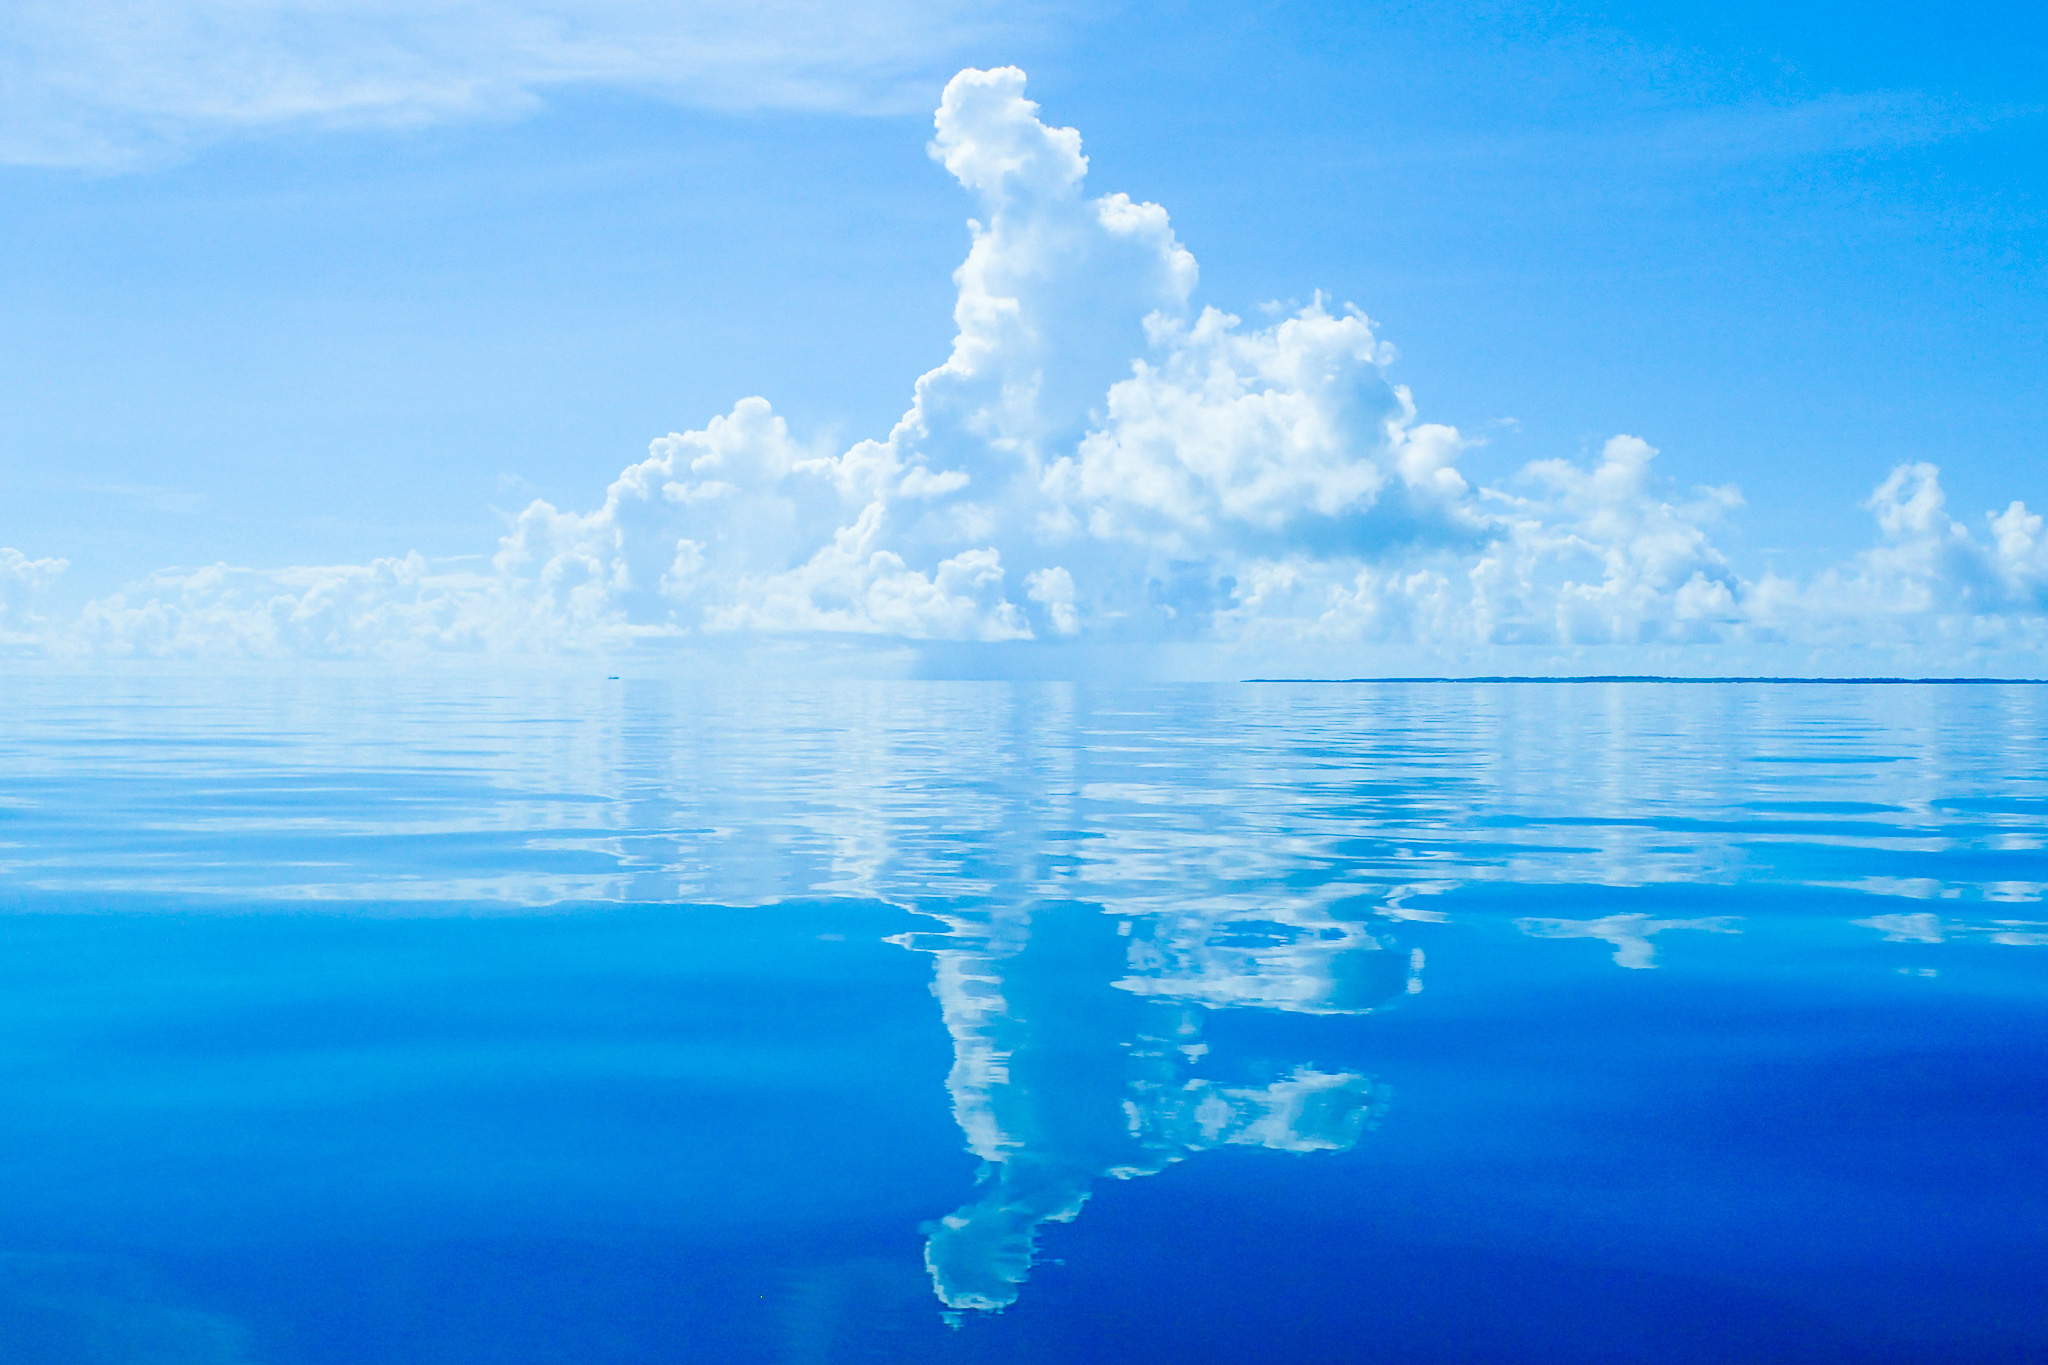
\includegraphics[width=\linewidth]{example.jpg}
        \caption{例1}
        \label{fig:ex1}
    \end{minipage}
    \hfill % 横の隙間を自動調整
    \begin{minipage}[b]{0.32\linewidth}
        \centering
        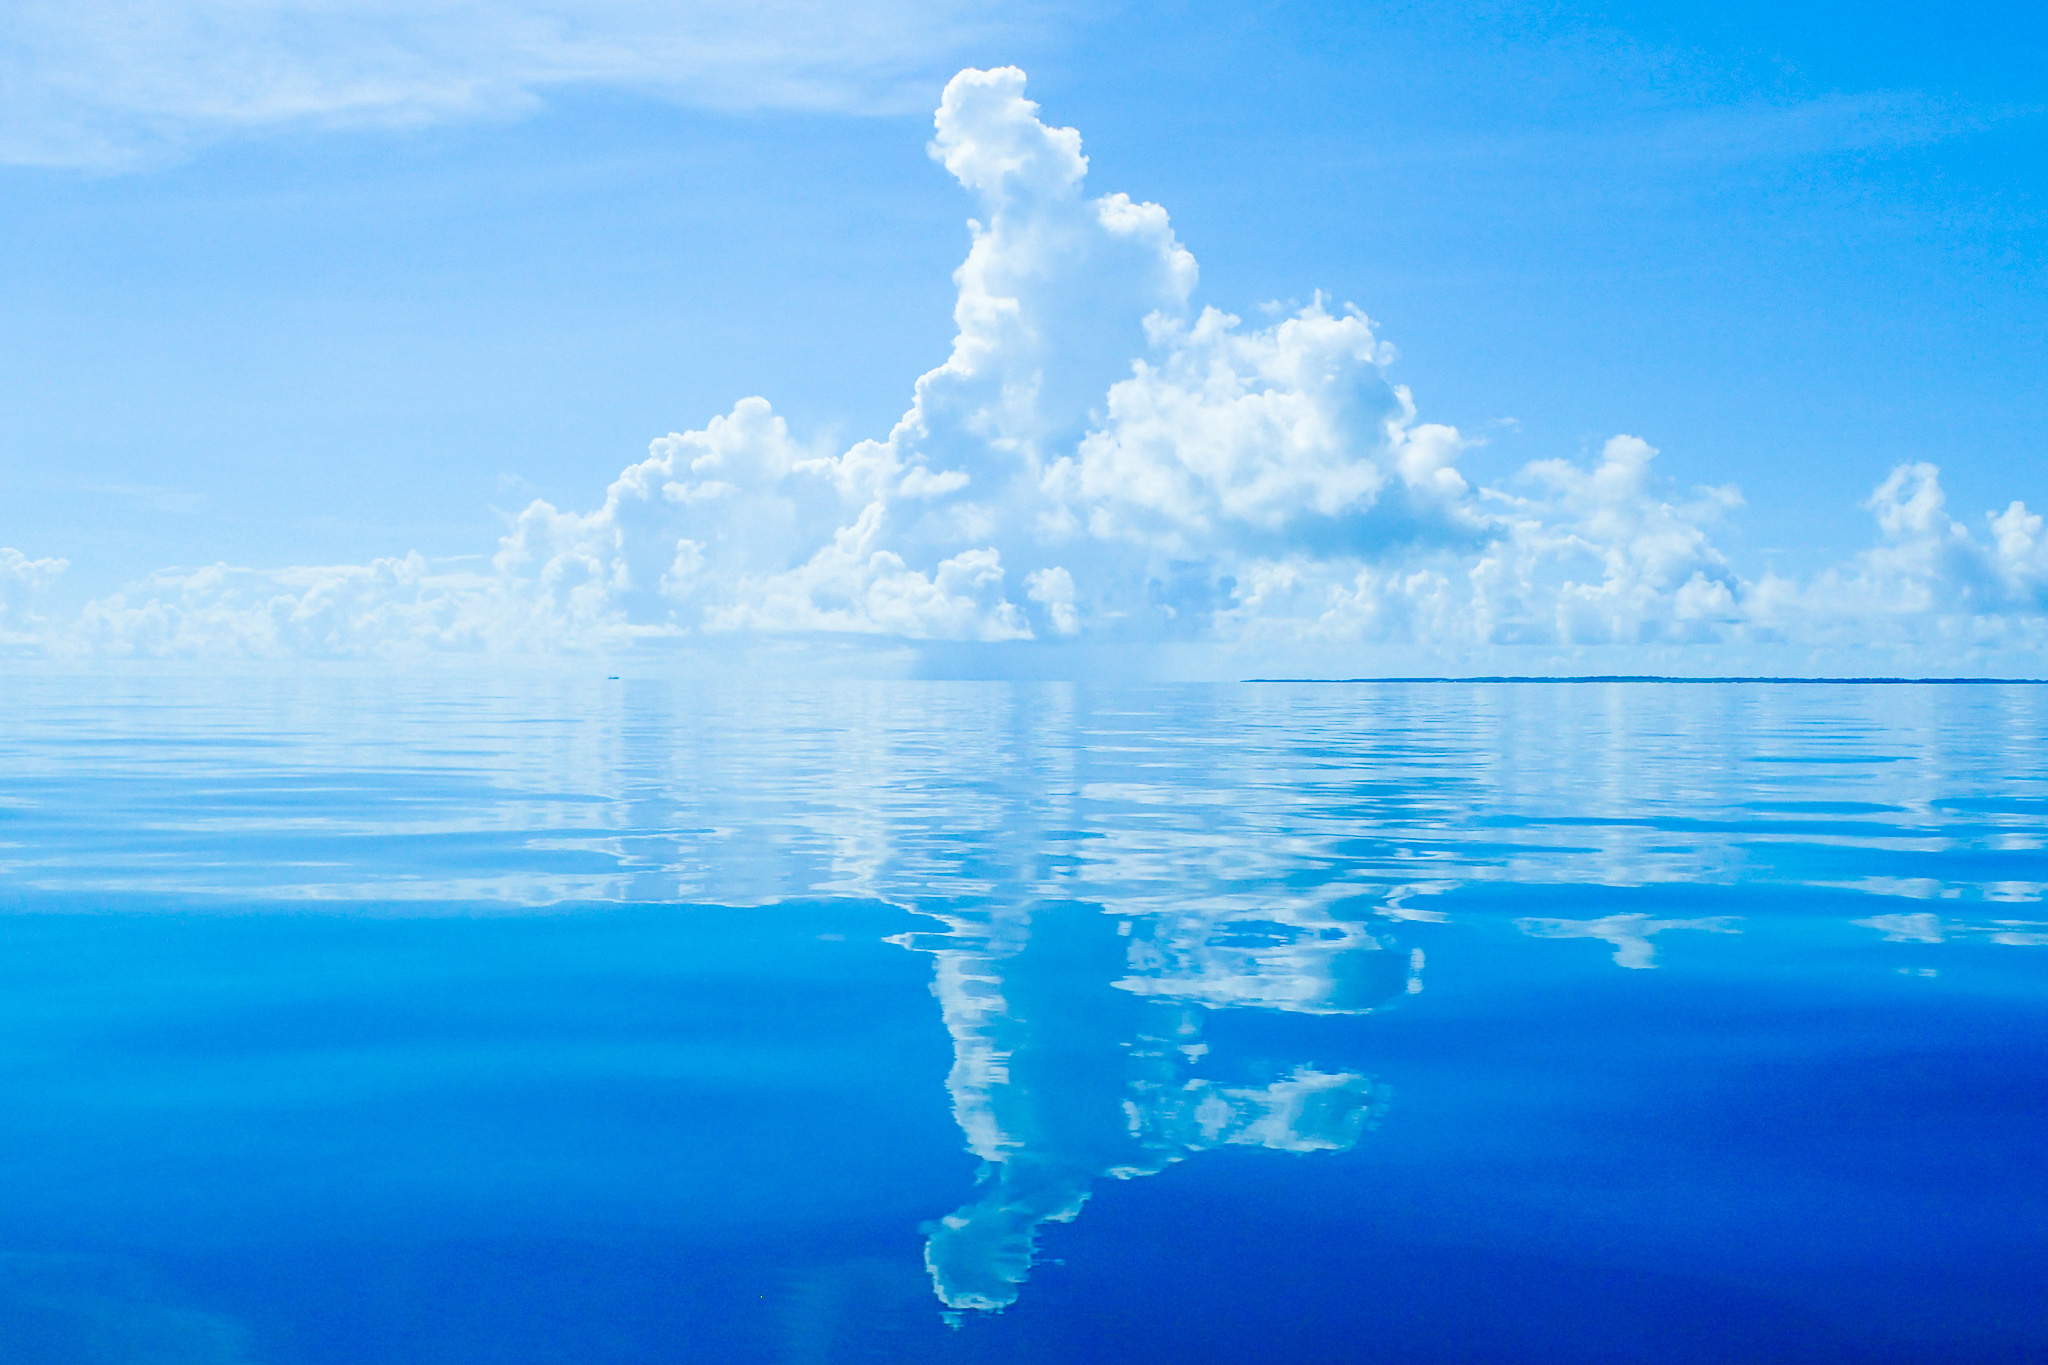
\includegraphics[width=\linewidth]{example.jpg}
        \caption{例2}
        \label{fig:ex2}
    \end{minipage}
    \hfill
    \begin{minipage}[b]{0.32\linewidth}
        \centering
        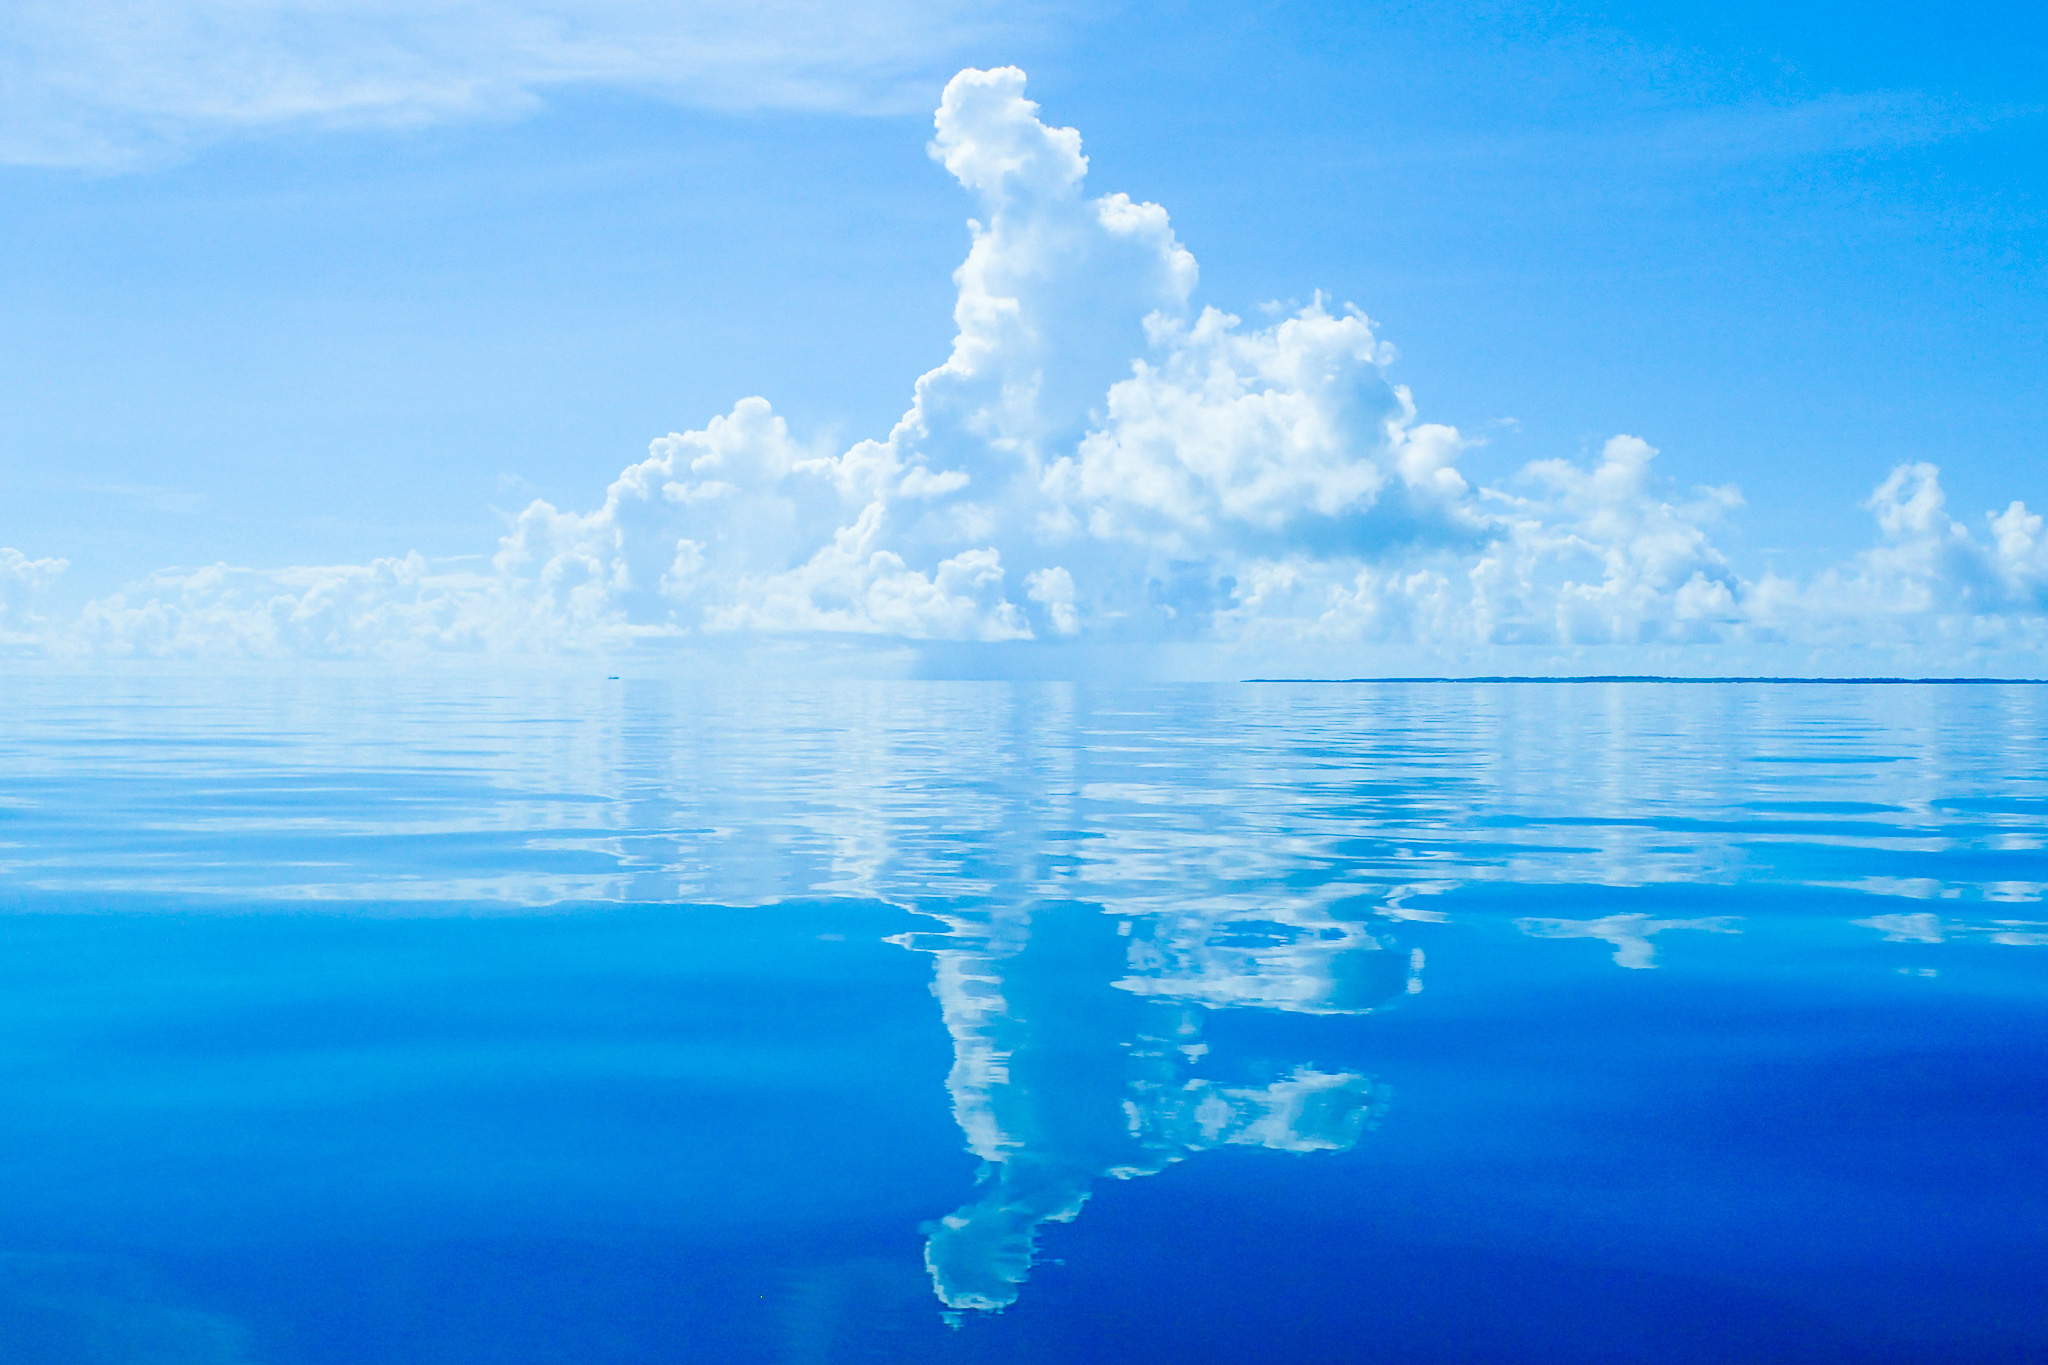
\includegraphics[width=\linewidth]{example.jpg}
        \caption{例3}
        \label{fig:ex3}
    \end{minipage}
\end{figure}
図\ref{fig:ex1}～図\ref{fig:ex3}は同じ画像ですが，このように複数の図を横並びで配置できます．

\section{表の挿入}
\begin{table}[H]
  \centering
  \caption{例の表}
  \label{tab:example}
  \begin{tabular}{|c|c|c|}
    \hline
    列1 & 列2 & 列3 \\
    \hline
    値1 & 値2 & 値3 \\
    \hline
  \end{tabular}
\end{table}
$\vert$c$\vert$c$\vert$r$\vert$ は列の配置（cは中央揃え、l/rは左/右揃え、$\vert$ は縦線）を表します。\\
\& で列を区切り、\textbackslash\textbackslash で改行します。\\
\textbackslash hline は横線を引きたいときに入れます。


\section{おわりに}
ここにまとめを書きます．

% === 参考文献の設定 ===
% 日本語文献が多い場合は junsrt や jaeet などのスタイルもおすすめです
\bibliographystyle{IEEEbib} 
\bibliography{reference} 

\end{document}